\documentclass{article}
\usepackage{graphicx}
\usepackage[margin=1.5cm]{geometry}
\usepackage{amsmath}

\begin{document}
\twocolumn

\title{Friday Warm Up: Unit 1, DC Circuits and Error Propagation}
\author{Prof. Jordan C. Hanson}

\maketitle

\section{Memory Bank}

\begin{itemize}
\item $V = IR$ ... The macroscopic version of Ohm's law
\item $R = L/(\sigma A)$ ... The resistance.  Units: $\Omega$.
\item $R_{\rm tot} = R_1 + R_2$ ... Resistors in series.
\item $R_{\rm tot}^{-1} = R_1^{-1} + R_2^{-1}$ ... Resistors in parallel.
\item $V_{\rm terminal} = \mathcal{E} - Ir$ ... The terminal voltage on a battery with emf $\mathcal{E}$, current $I$, and \textit{internal resistance} $r$.
\item $P = IV = I^2 R = V^2/R$ ... Expressions for the power in a DC circuit.
\item $(R_1 \pm \sigma_1) + (R_2 \pm \sigma_2) = (R_1 + R_2) \pm \sqrt{\sigma_1^2 + \sigma_2^2}$ Adding two measurements with associated errors.
\end{itemize}

\section{Ohm's Law and DC Circuits}

\begin{enumerate}
\item A battery with a 1.5 V emf powers a 15 $\Omega$ load, and has an internal resistance of $r = 1$ $\Omega$.  (a) What is total resistance in the circuit? (b) What current flows? (c) What is the terminal voltage? (d) If the battery has 150 mA hr of charge, how long will the battery power the circuit? \\ \vspace{5cm}
\item An 1800-W toaster, a 1400-W speaker, and a 75-W lamp are plugged into the same outlet in a 15-A fuse and 120-V circuit. (The three devices are in parallel when plugged into the same socket.) (a) What current is drawn by each device? (b) Will this combination blow the 15-A fuse? \\ \vspace{5cm}
\end{enumerate}

\section{Error Propagation}

\begin{enumerate}
\item Consider Fig. \ref{fig:1}.  The values of each resistor are quoted in Tab. \ref{tab:1}, along with associated errors.  What is the total resistance, with its associated error? \\ \vspace{4cm}
\item Suppose the circuit in Fig. \ref{fig:1} was given a voltage of 15 V (negligible imprecision).  What current would flow?  In your response account for the error in total resistance.
\end{enumerate}

\begin{figure}
\centering
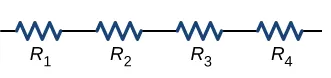
\includegraphics[width=0.35\textwidth]{figures/fourSeries.png}
\caption{\label{fig:1} Four resistors in series.}
\end{figure}

\begin{table}
\centering
\begin{tabular}{| c | c | c |}
\hline
\textbf{Resistor} & \textbf{Resistance} & \textbf{Error} \\
$R_1$ & 1.00 k$\Omega$ & 50 $\Omega$ \\
$R_1$ & 0.95 k$\Omega$ & 50 $\Omega$ \\
$R_1$ & 1.05 k$\Omega$ & 50 $\Omega$ \\
$R_1$ & 0.95 k$\Omega$ & 50 $\Omega$ \\
\hline
\end{tabular}
\caption{\label{tab:1} The resistances, with associated errors, for the resistors in Fig. \ref{fig:1}.}
\end{table}

\end{document}
